\section{Velocity Controller}\label{sec:velocityController}


\subsection{P-Controller}

% Calculating gain for half the time-constant, why, dunno?

% flowchart of code?

% Comparing step-response, P-controller and P-controller with feed-forward.
 \begin{figure}[H]
 	\centering
 	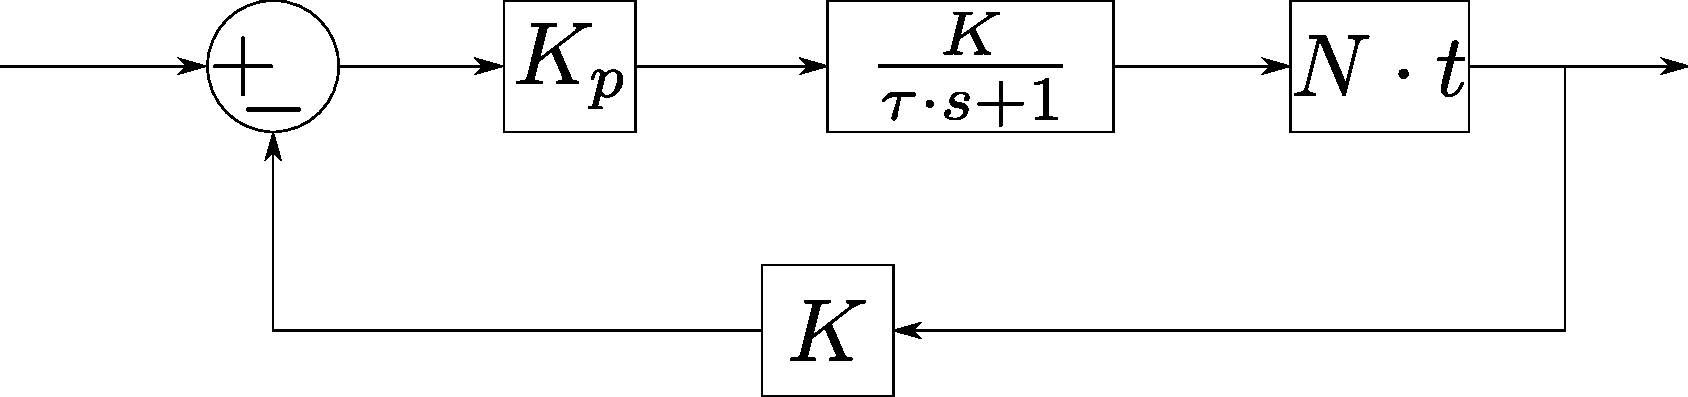
\includegraphics[scale=0.4]{figures/proportionalController.pdf}
 	\caption{Diagram of the proportional controller}
 	\label{proportionalController}
 \end{figure}
 
  \begin{figure}[H]
  	\centering
  	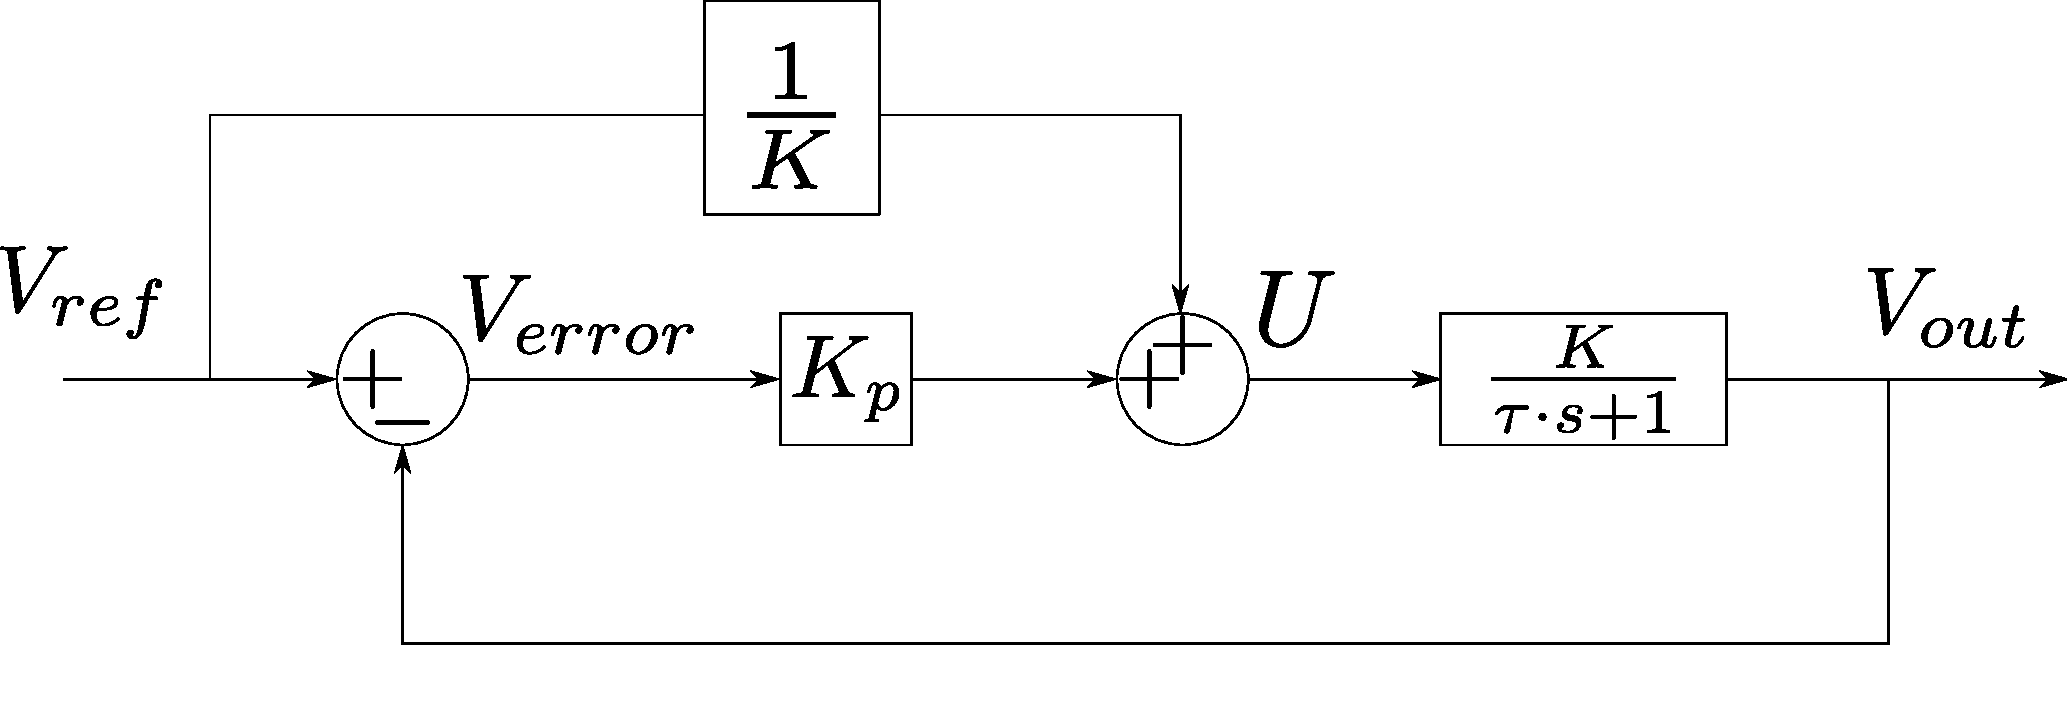
\includegraphics[scale=0.4]{figures/proportionalControllerWithFeedforward.pdf}
  	\caption{Diagram of the proportional controller with feedforward}
  	\label{proportionalControllerWithFeedforward}
  \end{figure}
 
% Results:
% Overshoot

% Conclusion: 
% That we need more than a P-controller, because of the overshoot. 




\subsection{PI-Controller}

  \begin{figure}[H]
  	\centering
  	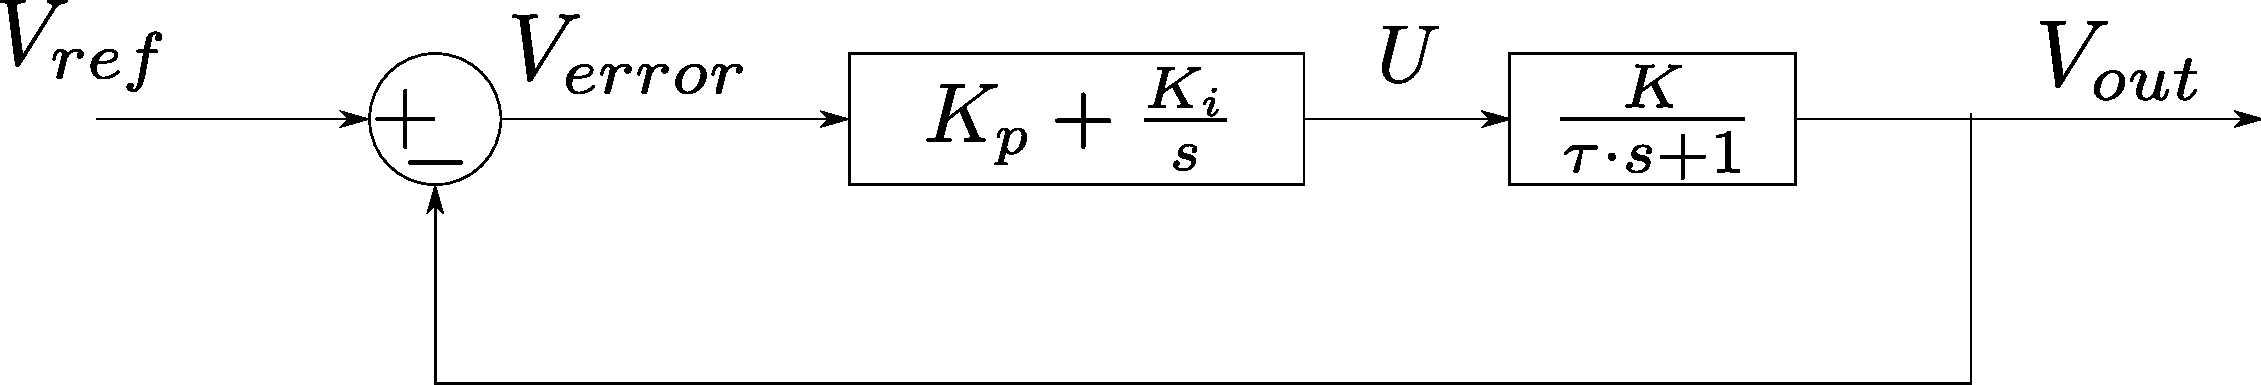
\includegraphics[scale=0.4]{figures/proportionalIntegratorController.pdf}
  	\caption{Diagram of the proportional and Integrator controller without feedforward}
  	\label{proportionalIntegratorController}
  \end{figure}